% ============================================================
%  Figuras del capítulo 1 del libro digital.
%  Cada tikzpicture sale en su propia página; después se
%  convierten a SVG con:  pdftocairo -svg -f N -l N figuras-cap01.pdf
%  Compilar con pdfLaTeX.
% ============================================================
\documentclass[tikz,border=3pt]{standalone}
\usepackage[T1]{fontenc}
\usepackage{amsmath,amssymb}
\usetikzlibrary{arrows.meta,calc}
\definecolor{turquesaGA}{HTML}{0E7C8C}
\definecolor{turquesaClaro}{HTML}{E2F2F4}
\definecolor{grisT}{HTML}{5F5E5A}
\definecolor{negroP}{HTML}{2B2B2B}
\definecolor{terracota}{HTML}{C1502E}
\definecolor{dorado}{HTML}{B07C10}
\begin{document}

% ---------- 1. Distancia del origen a un punto, en el plano ----------
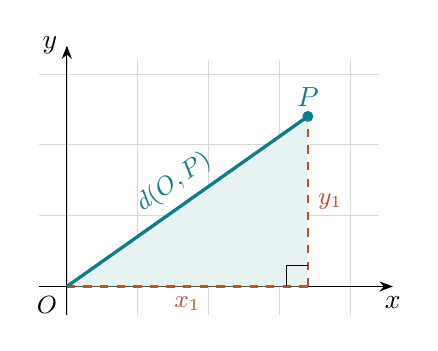
\begin{tikzpicture}[scale=.9,>=Stealth]
  \draw[very thin,color=gray!30] (-0.4,-0.4) grid (4.4,3.2);
  \draw[->] (-0.4,0) -- (4.6,0) node[below]{$x$};
  \draw[->] (0,-0.4) -- (0,3.4) node[left]{$y$};
  \coordinate (O) at (0,0);
  \coordinate (P) at (3.4,2.4);
  \coordinate (R) at (3.4,0);
  \fill[turquesaGA!10] (O) -- (R) -- (P) -- cycle;
  \draw[dashed,terracota,thick] (O) -- (R) node[midway,below]{\small $x_1$};
  \draw[dashed,terracota,thick] (R) -- (P) node[midway,right]{\small $y_1$};
  \draw[turquesaGA,very thick] (O) -- (P)
    node[midway,above,sloped]{\small $d(O,P)$};
  \draw (3.1,0) -- (3.1,0.3) -- (3.4,0.3);
  \fill[turquesaGA] (P) circle(2.2pt) node[above]{$P$};
  \node[below left,font=\small] at (O) {$O$};
\end{tikzpicture}

% ---------- 2. El mismo triángulo, fuera del origen ----------
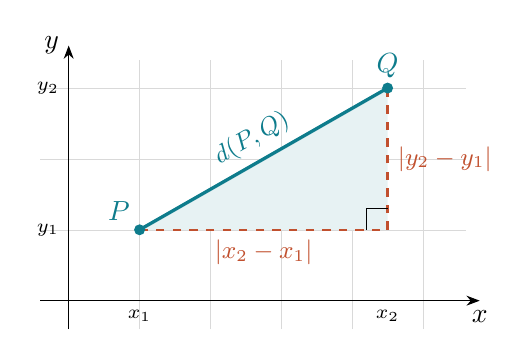
\begin{tikzpicture}[scale=.9,>=Stealth]
  \draw[very thin,color=gray!30] (-0.4,-0.4) grid (5.6,3.4);
  \draw[->] (-0.4,0) -- (5.8,0) node[below]{$x$};
  \draw[->] (0,-0.4) -- (0,3.6) node[left]{$y$};
  \coordinate (P) at (1,1);
  \coordinate (Q) at (4.5,3);
  \coordinate (R) at (4.5,1);
  \node[below,font=\scriptsize] at (1,0) {$x_1$};
  \node[below,font=\scriptsize] at (4.5,0) {$x_2$};
  \node[left,font=\scriptsize] at (0,1) {$y_1$};
  \node[left,font=\scriptsize] at (0,3) {$y_2$};
  \fill[turquesaGA!10] (P) -- (R) -- (Q) -- cycle;
  \draw[turquesaGA,very thick] (P) -- (Q)
    node[midway,above,sloped]{\small $d(P,Q)$};
  \draw[dashed,terracota,thick] (P) -- (R)
    node[midway,below]{\small $|x_2-x_1|$};
  \draw[dashed,terracota,thick] (R) -- (Q)
    node[midway,right]{\small $|y_2-y_1|$};
  \draw (4.2,1) -- (4.2,1.3) -- (4.5,1.3);
  \fill[turquesaGA] (P) circle(2.2pt) node[above left]{$P$};
  \fill[turquesaGA] (Q) circle(2.2pt) node[above]{$Q$};
\end{tikzpicture}

% ---------- 3. Distancia del origen a un punto, en el espacio ----------
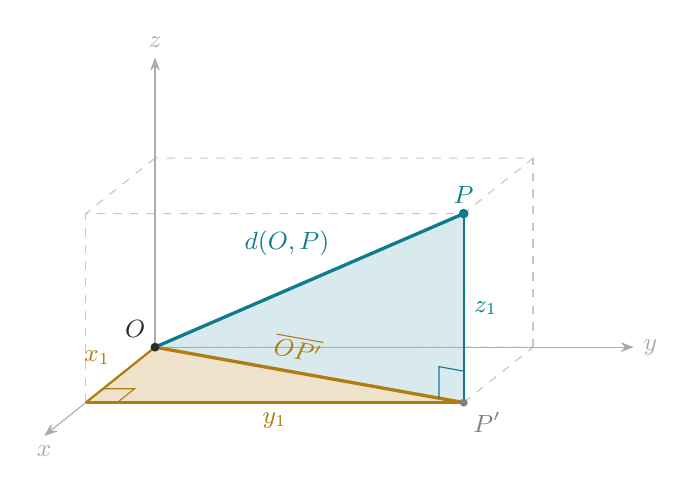
\begin{tikzpicture}[x={(-0.55cm,-0.44cm)},y={(1cm,0cm)},z={(0cm,1cm)},
                    scale=0.8,>=Stealth]
  \fill[dorado!22] (0,0,0) -- (2,0,0) -- (2,6,0) -- cycle;
  \fill[turquesaGA!16] (0,0,0) -- (2,6,0) -- (2,6,3) -- cycle;
  \draw[gray!45,dashed] (2,6,0) -- (0,6,0) -- (0,0,0);
  \draw[gray!45,dashed] (0,0,3) -- (2,0,3) -- (2,6,3) -- (0,6,3) -- cycle;
  \draw[gray!45,dashed] (0,0,0) -- (0,0,3);
  \draw[gray!45,dashed] (2,0,0) -- (2,0,3);
  \draw[gray!45,dashed] (0,6,0) -- (0,6,3);
  \draw[->,gray!65] (0,0,0) -- (3.2,0,0) node[below,font=\small]{$x$};
  \draw[->,gray!65] (0,0,0) -- (0,7.6,0) node[right,font=\small]{$y$};
  \draw[->,gray!65] (0,0,0) -- (0,0,4.6) node[above,font=\small]{$z$};
  \draw[dorado,thick] (0,0,0) -- (2,0,0)
    node[midway,above left,font=\small]{$x_1$};
  \draw[dorado,thick] (2,0,0) -- (2,6,0)
    node[midway,below,font=\small]{$y_1$};
  \draw[dorado,very thick] (0,0,0) -- (2,6,0)
    node[pos=0.45,above,sloped,font=\small,yshift=1pt]{$\overline{OP'}$};
  \draw[dorado] (1.5,0,0) -- (1.5,0.5,0) -- (2,0.5,0);
  \draw[turquesaGA,thick] (2,6,0) -- (2,6,3)
    node[midway,right,font=\small]{$z_1$};
  \draw[turquesaGA,very thick] (0,0,0) -- (2,6,3)
    node[pos=0.6,above left,font=\small]{$d(O,P)$};
  \draw[turquesaGA] (1.84,5.52,0) -- (1.84,5.52,0.5) -- (2,6,0.5);
  \fill[negroP] (0,0,0) circle(2pt) node[above left,font=\small]{$O$};
  \fill[turquesaGA] (2,6,3) circle(2.2pt) node[above,font=\small]{$P$};
  \fill[gray] (2,6,0) circle(1.8pt) node[below right,font=\small]{$P'$};
\end{tikzpicture}

% ---------- 4. Distancia entre dos puntos del espacio ----------
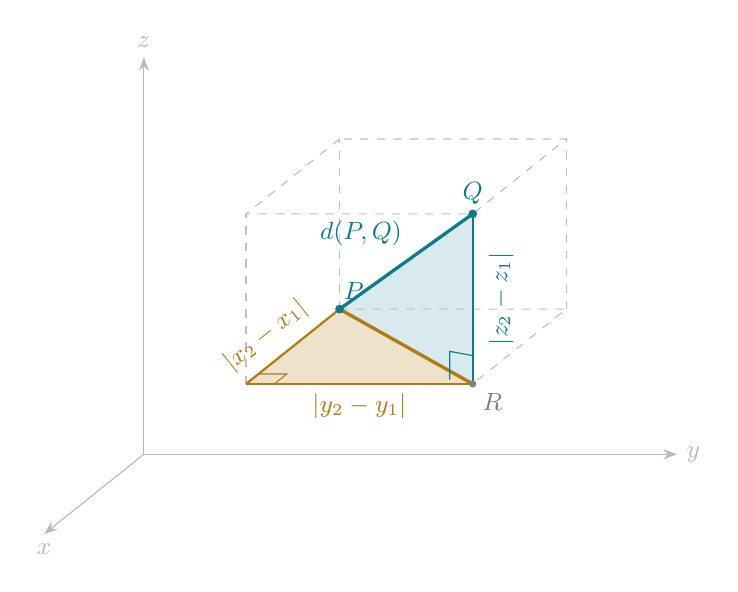
\begin{tikzpicture}[x={(-0.55cm,-0.44cm)},y={(1cm,0cm)},z={(0cm,1cm)},
                    scale=0.72,>=Stealth]
  \fill[dorado!22] (1,4,3) -- (4,4,3) -- (4,8,3) -- cycle;
  \fill[turquesaGA!16] (1,4,3) -- (4,8,3) -- (4,8,6) -- cycle;
  \draw[gray!50,dashed] (1,4,6) -- (4,4,6) -- (4,8,6) -- (1,8,6) -- cycle;
  \draw[gray!50,dashed] (1,4,3) -- (1,4,6);
  \draw[gray!50,dashed] (4,4,3) -- (4,4,6);
  \draw[gray!50,dashed] (1,8,3) -- (1,8,6);
  \draw[gray!50,dashed] (1,4,3) -- (1,8,3) -- (4,8,3);
  \draw[->,gray!55] (0,0,0) -- (3.2,0,0) node[below,font=\small]{$x$};
  \draw[->,gray!55] (0,0,0) -- (0,9.4,0) node[right,font=\small]{$y$};
  \draw[->,gray!55] (0,0,0) -- (0,0,7) node[above,font=\small]{$z$};
  \draw[dorado,thick] (1,4,3) -- (4,4,3)
    node[pos=0.62,above,sloped,font=\small,yshift=1pt]{$|x_2-x_1|$};
  \draw[dorado,thick] (4,4,3) -- (4,8,3)
    node[midway,below,font=\small]{$|y_2-y_1|$};
  \draw[dorado,very thick] (1,4,3) -- (4,8,3);
  \draw[dorado] (3.6,4,3) -- (3.6,4.5,3) -- (4,4.5,3);
  \draw[turquesaGA,thick] (4,8,3) -- (4,8,6)
    node[midway,below,sloped,font=\small,yshift=-2pt]{$|z_2-z_1|$};
  \draw[turquesaGA,very thick] (1,4,3) -- (4,8,6)
    node[pos=0.55,above left,font=\small]{$d(P,Q)$};
  \draw[turquesaGA] (3.83,7.5,3) -- (3.83,7.5,3.5) -- (4,8,3.5);
  \fill[turquesaGA] (1,4,3) circle(2.2pt)
    node[above right,font=\small,xshift=-2pt]{$P$};
  \fill[turquesaGA] (4,8,6) circle(2.2pt) node[above,font=\small]{$Q$};
  \fill[gray] (4,8,3) circle(1.8pt) node[below right,font=\small]{$R$};
\end{tikzpicture}

% ---------- 5. Los ocho octantes ----------
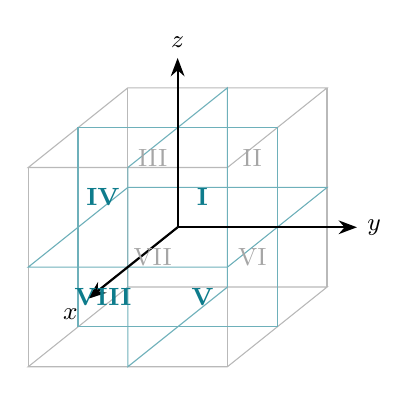
\begin{tikzpicture}[scale=1.15,>=Stealth]
  \draw[gray!55] (0.55,0.66) -- (1.65,1.54) -- (-0.55,1.54) -- (-1.65,0.66) -- cycle;
  \draw[gray!55] (0.55,-1.54) -- (1.65,-0.66) -- (-0.55,-0.66) -- (-1.65,-1.54) -- cycle;
  \draw[gray!55] (0.55,0.66) -- (0.55,-1.54);
  \draw[gray!55] (1.65,1.54) -- (1.65,-0.66);
  \draw[gray!55] (-0.55,1.54) -- (-0.55,-0.66);
  \draw[gray!55] (-1.65,0.66) -- (-1.65,-1.54);
  \draw[turquesaGA!60,thin] (0.55,-0.44) -- (1.65,0.44) -- (-0.55,0.44) -- (-1.65,-0.44) -- cycle;
  \draw[turquesaGA!60,thin] (-0.55,0.66) -- (0.55,1.54) -- (0.55,-0.66) -- (-0.55,-1.54) -- cycle;
  \draw[turquesaGA!60,thin] (1.1,1.1) -- (-1.1,1.1) -- (-1.1,-1.1) -- (1.1,-1.1) -- cycle;
  \draw[->,thick] (0,0) -- (-0.99,-0.79) node[below left,font=\small]{$x$};
  \draw[->,thick] (0,0) -- (1.98,0) node[right,font=\small]{$y$};
  \draw[->,thick] (0,0) -- (0,1.87) node[above,font=\small]{$z$};
  \node[font=\small\bfseries,color=turquesaGA] at (0.275,0.33) {I};
  \node[font=\small,color=gray!70] at (0.825,0.77) {II};
  \node[font=\small,color=gray!70] at (-0.275,0.77) {III};
  \node[font=\small\bfseries,color=turquesaGA] at (-0.825,0.33) {IV};
  \node[font=\small\bfseries,color=turquesaGA] at (0.275,-0.77) {V};
  \node[font=\small,color=gray!70] at (0.825,-0.33) {VI};
  \node[font=\small,color=gray!70] at (-0.275,-0.33) {VII};
  \node[font=\small\bfseries,color=turquesaGA] at (-0.825,-0.77) {VIII};
\end{tikzpicture}

% ---------- 6. Los tres planos coordenados ----------
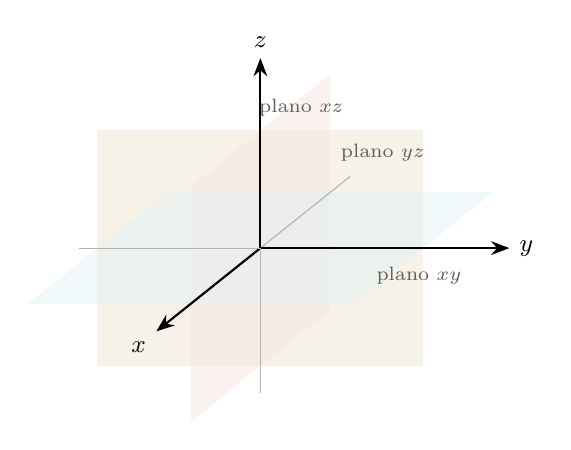
\begin{tikzpicture}[scale=1.15,>=Stealth]
  \fill[dorado!20,opacity=0.5] (-1.8,-1.3) rectangle (1.8,1.3);
  \fill[terracota!15,opacity=0.5]
    (-0.77,0.68) -- (0.77,1.92) -- (0.77,-0.68) -- (-0.77,-1.92) -- cycle;
  \fill[turquesaClaro,opacity=0.5]
    (1.03,-0.62) -- (2.57,0.62) -- (-1.03,0.62) -- (-2.57,-0.62) -- cycle;
  \draw[->,thick] (0,0) -- (-1.15,-0.92) node[below left,font=\small]{$x$};
  \draw[gray!60] (0,0) -- (0.99,0.79);
  \draw[->,thick] (0,0) -- (2.75,0) node[right,font=\small]{$y$};
  \draw[gray!60] (0,0) -- (-2.0,0);
  \draw[->,thick] (0,0) -- (0,2.1) node[above,font=\small]{$z$};
  \draw[gray!60] (0,0) -- (0,-1.6);
  \node[font=\scriptsize,color=grisT] at (1.75,-0.30) {plano $xy$};
  \node[font=\scriptsize,color=grisT] at (1.35,1.05) {plano $yz$};
  \node[font=\scriptsize,color=grisT] at (0.45,1.55) {plano $xz$};
\end{tikzpicture}

\end{document}
